\documentclass[10pt]{article}

\usepackage{cmap}
\usepackage[T2A]{fontenc}
\usepackage[utf8]{inputenc}
\usepackage[russian]{babel}
\usepackage{graphicx}
\usepackage{amsthm,amsmath,amssymb}
\usepackage[russian,colorlinks=true,urlcolor=blue,linkcolor=blue]{hyperref}
\usepackage{enumerate}
\usepackage{datetime}
\usepackage{fancyhdr}
\usepackage{lastpage}
\usepackage{enumitem}
\usepackage{xcolor}
\usepackage{graphicx}
\usepackage{graphbox}

% Setup colours for links
\definecolor{linkcolour}{rgb}{0,0.2,0.6}
\hypersetup{colorlinks,breaklinks,urlcolor=linkcolour, linkcolor=linkcolour}


\parskip=0em
\parindent=0em

\sloppy
\voffset=-30mm
\textheight=250mm
\hoffset=-30mm
\textwidth=180mm
\headsep=11pt
\footskip=-10pt


% Indentation
\def\makeparindent{\hspace*{\parindent}}
\def\up{\vspace*{-\baselineskip}}
\def\down{\vspace*{\baselineskip}}
\def\LINE{\vspace*{-1em}\noindent \underline{\hbox to 1\textwidth{{ } \hfil{ } \hfil{ } }}}

\pagenumbering{gobble}

\definecolor{accent}{RGB}{64, 0, 128}

\begin{document}


%--------------------TITLE-------------

\begin{tabular}{rlll}
       {\bf \huge Dmitrii Abramov} &  \  & location: &Saint Petersburg, Russia\\ 
    \textsc{\color{accent} Software Engineer} & \ & phone / telegram:   & +7 999 227 15 45\\
    & \ & e-mail:             & \href{mailto:dmitrii.abramov@outlook.com}{dmitrii.abramov@outlook.com}\\
    & \ & github:             & \href{https://github.com/karvozavr}{github.com/karvozavr}\\
   & \ &   \                 & \href{https://www.linkedin.com/in/dmitriy-abramov/}{LinkedIn}  
\end{tabular}
 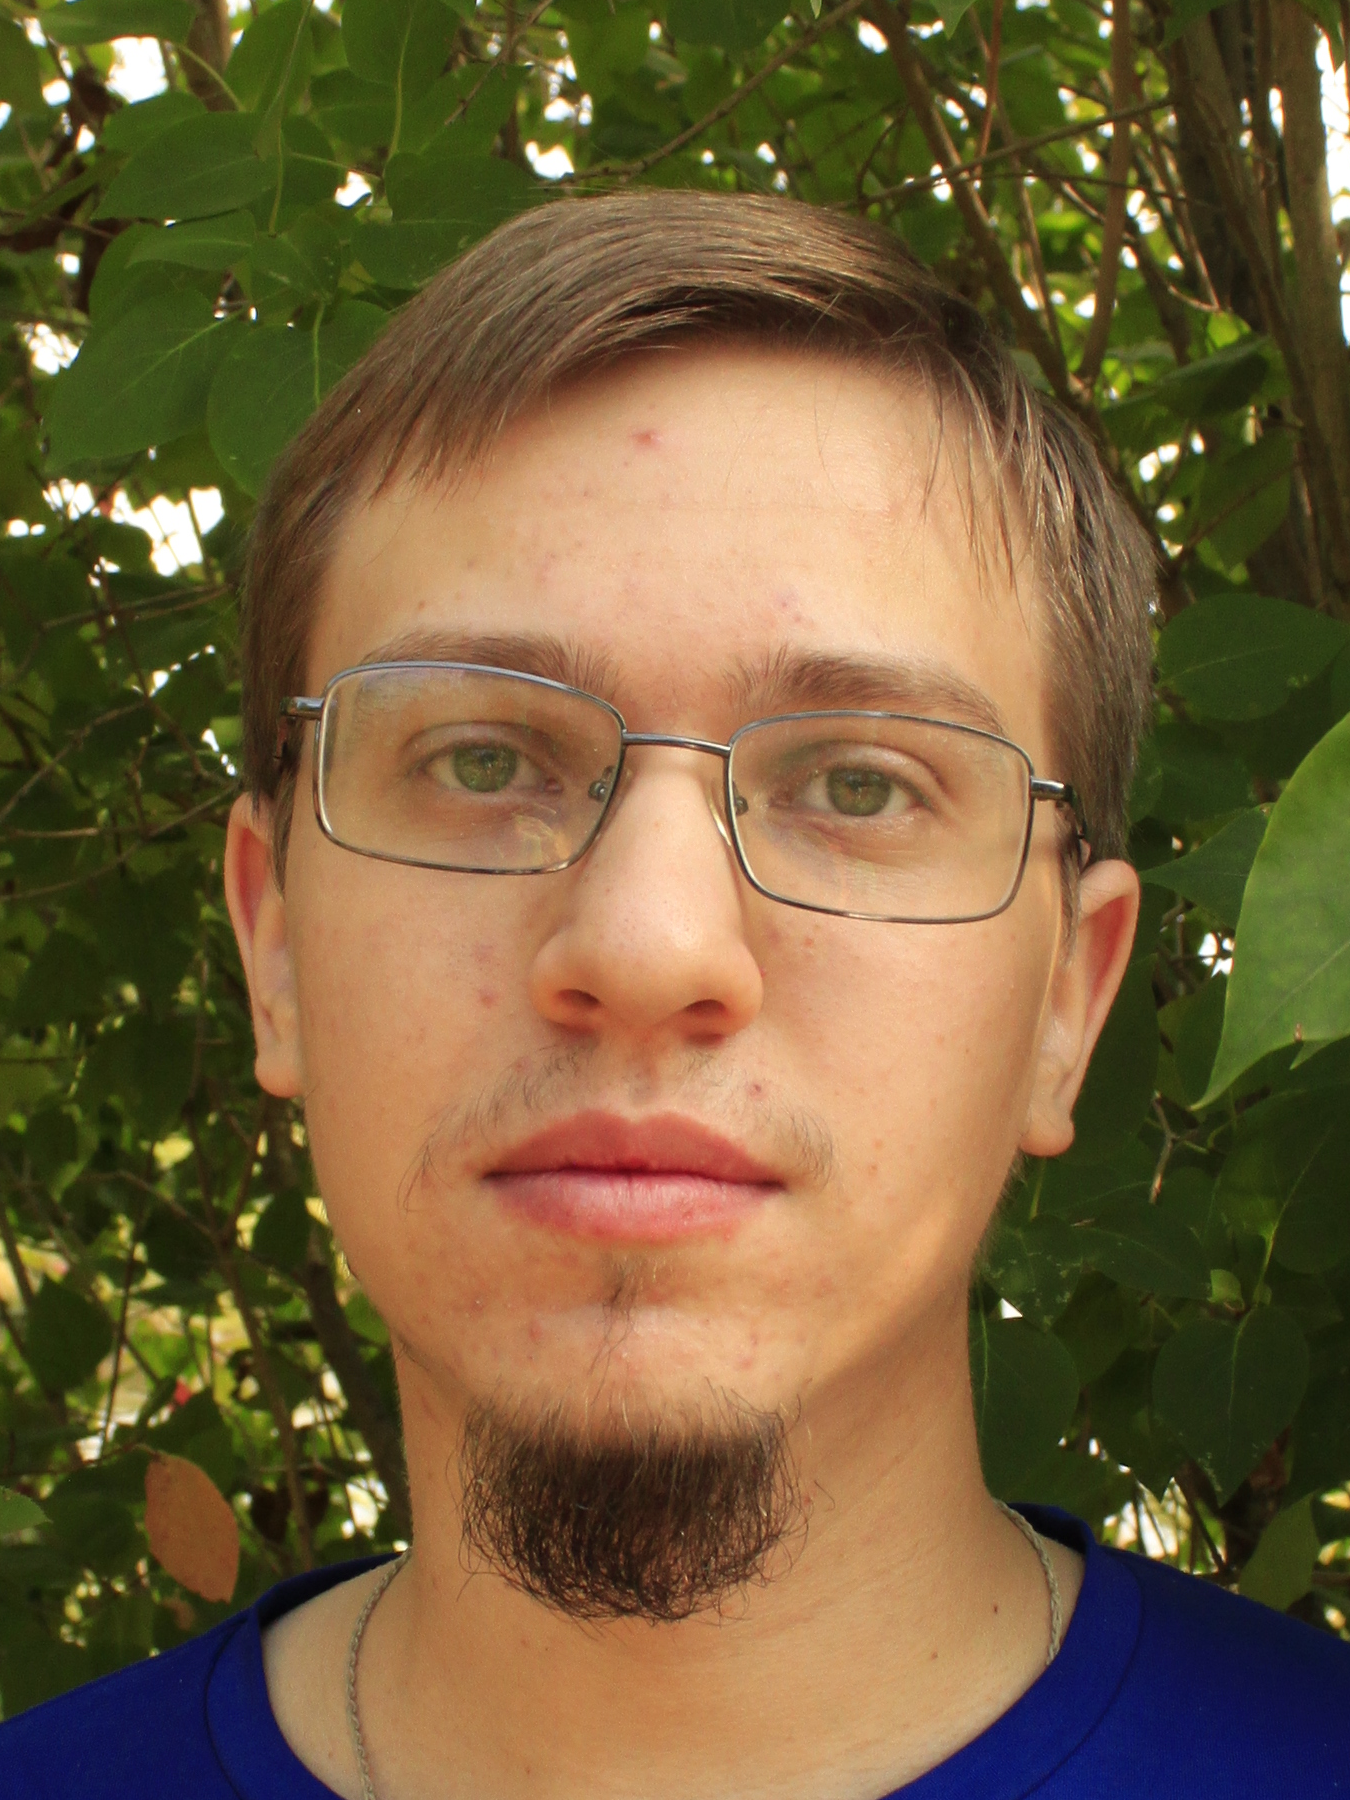
\includegraphics[align=c, scale=0.05]{me.png} 
 \\
\LINE

\section*{\color{accent} Education}
\begin{tabular}{rl}
 \textsc{2016-2020} & \textbf{Higher School of Economics}, Saint Petersburg, Russia\\
 \  & Bachelor of Science in \textsc{Computer Science}
\end{tabular}
% \begin{itemize} 

%     \item \footnotesize{Passed classes: Software Design, Algorithms and Data Structures, 
%           Computer Networking, Machine Learning, Compilers, Operating Systems, 
%           Discrete Math, Programming Paradigms, UNIX,
%           Statistics, Lambda Calculus and Functional Programming, 
%           Type Theory, Formal Languages.}

% \end{itemize}

\  \\

\LINE
\section*{\color{accent} Work experience}
\begin{tabular}{p{2.5cm}|p{14cm}}

  Summer 2019 & \textbf{Deutsche Bank Technology Centre} \\
    & \emph{Software Engineer at Test (intern)}\\
  & \footnotesize{Designing, creating and enchancing testing tools for several Bank projects. \newline I've been working with such technologies as: Spring, Apache Kafka, Oracle DB, Cucumber BDD, Angular.}\\
  \\
   \  & \textbf{Summer Informatics School}, Russia \\
   2017 - Now &\emph{Teacher}\\
   \  &\footnotesize{Teaching Python, algorithms and data structures to high school students.}\\\multicolumn{2}{c}{} \\
\end{tabular}
\\
\LINE
\section*{\color{accent} Projects}
\begin{tabular}{p{2.5cm}|p{14.7cm}}
  April-May 2017 \  & \textbf{ROS Map Generator} \href{https://github.com/karvozavr/ROS-Map-Generator}{\scriptsize (github)} \\
  & \footnotesize{I have implemented tool for generation of random maps, which represent environment used for robots' navigation systems in ROS project (open source robotic software). Generated maps are being exported to specific format that can be used with ROS map server. The resulting generator tool can be used for testing SLAM algorithms. Project implemented in \textsc{C++14}.}  \\
  % &How it works: generate set of rooms of random size, separate them using separation steering, delete half of rooms to create some free space.
  % Build a relative neighborhood graph on those rooms using naive triangulation.
  % Then connect every pair of rooms, that has an edge in the graph with corridor.
  % At the end, render the rooms and save the resulting environment map to ROS map\_server compatible format (pgm image + YAML).
  Fall 2017  & \textbf{CityQuest} \href{https://github.com/karvozavr/CityQuest/tree/dev}{\scriptsize (github)} \\
  & \footnotesize{This is a service for outdoor quests in reality. I`ve been managing teamwork process and implemented Android application for passing quests. I used Google Drive API and Google Auth for user accounts system and storing and sharing user progress. 
    App supports various types of quest task and it`s functionality can be easily extended. The entire app is implemented using Java and Android API.}   \\
  Spring 2018 & \textbf{Dota Deep-RL with demonstrations} \href{https://github.com/karvozavr/DotA-DeepRL}{\scriptsize (github)} \\
  & \footnotesize{This is a research project about how deep reinforcement learning with demonstrations method may be applied to a complex environment like Dota 2 game.}   \\
    October 2018 - & \textbf{After Effects PinTool plugin} \\
  May 2019 & \footnotesize{As a part of \href{https://www.keentools.io/}{KeenTools} team, I've been implementing version of PinTool plugin for Adobe After Effects. I've implemented integration with After Effects, custom rendering engine and positioning system.} \\
  Spring 2019 & \textbf{BIOCAD intelligent production scheduling} \\
  & \footnotesize{I've participated in Hackuniversity (All-Russian University Hackathon). The project of my team was creating the tool for production schedule optimisation and schedule management. I've implemented data processing, schedule building algorithm, backend in Python and deployed it in the cloud (AWS) along with Postgres DB.}  
\end{tabular}
\\
\LINE
\section*{\color{accent} Skills and Technologies}
\begin{itemize}[font=\bfseries,  wide=1.5em,  leftmargin=*]
  \item[Used in projects:] \  \\ Java, Kotlin, Spring, Python, SQL, C++.
  \item[Classroom experience:] \ \\ Scala, Haskell, OCaml, C, Bash, Android, AWS, x86 Assembly, Go, JavaScript, HTML/CSS.
  \item[Tools:] \ \\ Docker, Git, Tensorflow, Linux, Jenkins, \LaTeX.
\end{itemize}

\end{document}